\section{Length-Weighting Derivation}
\label{app:normalization}

Fix a rollout batch, its valid-token masks, and domain weights $\lambda_d$. Any PG coefficients are detached. For $n_d=|\mathcal B_d|$, let $\bar T_d=n_d^{-1}\sum_{i\in\mathcal B_d}T_i$ and $\bar g_d=n_d^{-1}\sum_{i\in\mathcal B_d}g_i$. Define the empirical covariance using the same $1/n_d$ normalization:
\begin{equation}
\operatorname{Cov}_d(T,g)=\frac{1}{n_d}\sum_{i\in\mathcal B_d}(T_i-\bar T_d)(g_i-\bar g_d).
\end{equation}
Expanding gives $n_d^{-1}\sum_iT_i g_i-\bar T_d\bar g_d$. Dividing by $\bar T_d$ yields Equation~\ref{eq:weighting}. GT combines the resulting domain gradients using observed token shares; DT combines them using $\lambda_d$; DR combines $\bar g_d$ using $\lambda_d$. Multiplying each domain's globally averaged terms by its target weight divided by its observed token share therefore gives DT exactly.

The derivation is a finite-batch weighted-average identity. Response sampling, masks, and lengths are held fixed. Its population analogue involves an expectation of a ratio; replacing that expectation by a ratio of expectations requires additional assumptions or a large-batch limit.

\subsection{Fixed-batch gradient comparison}
\label{app:fixed_batch_normalization}

At M-PG checkpoints 100 and 250, three banks (seeds 1042, 1043, and 1044) each contain eight responses per domain. Responses use the training prompt format and 4,096-token response cap. For each bank, we compute each response's mean I64 gradient once at the saved BF16 model values using FP32 computation, then aggregate those gradients under DR, DT, and GT. All three reductions use the same responses, token masks, teacher scores, and model coordinates. Student and optimizer snapshots match within each checkpoint.

Table~\ref{tab:fixed_batch_normalization} reports every pairwise raw-gradient cosine. The domain-wise covariance decomposition is checked in FP64 over all 24 bank-domain groups; the largest relative residual is $1.53\times10^{-15}$. This numerical check verifies the aggregation identity. The observed gradient directions establish that the covariance contribution is nonzero on these batches.

\begin{table}[t]
\caption{Fixed-batch averaging comparison. Entries are raw-gradient cosines; each row uses one shared student and response bank. DR and DT share domain weights and differ only in within-domain response weighting.}
\label{tab:fixed_batch_normalization}
\centering\small
\begin{tabular}{rrrrr}
\toprule
Updates & Batch & DR--DT & DR--GT & DT--GT \\
\midrule
100 & 1 & 0.7838 & 0.6219 & 0.9266 \\
100 & 2 & 0.9110 & 0.5180 & 0.7010 \\
100 & 3 & 0.5780 & 0.6659 & 0.9745 \\
250 & 1 & 0.6240 & 0.4072 & 0.8742 \\
250 & 2 & 0.7864 & 0.3302 & 0.4953 \\
250 & 3 & 0.3990 & 0.3569 & 0.9612 \\
\bottomrule
\end{tabular}

\end{table}

\section{Parameter and Optimizer Measurements}
\label{app:records}

\subsection{Coordinates and recorded quantities}

The online record distinguishes raw aggregate gradients, clipped gradients, actual FP32 optimizer steps, cumulative FP32 master changes, and cumulative BF16 model changes. Cumulative changes use the same initialization reference. All global statistics use unique model coordinates, excluding vocabulary padding and shared duplicates. Per-layer statistics and absolute-threshold sensitivities are retained in the frozen measurements. The sparsity value is the fraction at or below a threshold; figures report its complement. Energy concentration uses squared Euclidean norm and ranks coordinates by absolute change.

For local calculations, the exported checkpoint contains FP32 master values, BF16 model values, first and second moments, optimizer hyperparameters, and step clocks. The BF16 values match all 1,720,574,976 coordinates in the native exported model. Teacher weight values are verified in the same precision. Local forward/backward computations evaluate these values in FP32 with TF32 disabled. All proposed steps are computed from the same saved state with a non-fused Adam implementation. The online training optimizer uses its own fused implementation.

We evaluate three local states. \emph{Saved} retains both moments and the step clock. \emph{Reset m} zeros the first moment while retaining the second moment and clock. \emph{Fresh} zeros both moments and resets the clock. Global norm clipping at 1 is applied before the Adam calculation, and weight decay is zero. For the zero-gradient branch, the saved first moment continues to decay and move the master weights. A no-step master-to-BF16 cast gives an exact match to the saved model. Thirteen numerical checks cover the Adam formulas against PyTorch, loss gradients, parameter-coordinate inner products, support ties, and zero-vector handling. Figure~\ref{fig:thresholds} shows how absolute thresholds change the measured local activity.

The zero-current-gradient branch changes 0.1403\% of BF16 coordinates, compared with 0.1486\% for PG. Resetting the first moment gives 0.0504\% for PG; resetting both moments and the clock gives 0.5140\%. These controls explain why a sparse gradient selection cannot by itself identify the parameters changed by an optimizer step. They supplement the update-sparsity measurements in Sections~\ref{sec:subnetworks} and~\ref{sec:density}.

\begin{figure}[t]
\centering
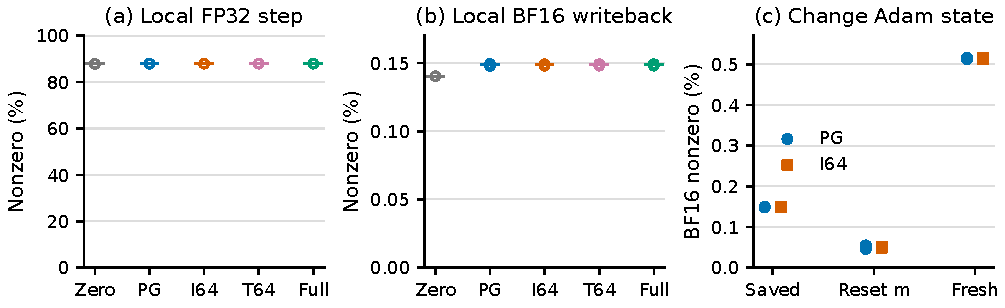
\includegraphics[width=\linewidth]{figures/aligned_evidence_20260910/adam_precision.pdf}
\caption{Supporting optimizer-state controls at M-PG update 100. Points show two response banks; the zero-gradient control is evaluated once. (a,b) Nonzero fractions for FP32 steps and BF16 changes. (c) Saved moments, reset first moment, and fresh moments and clock. Weight decay is zero.}
\label{fig:adam}
\end{figure}

\begin{figure}[t]
\centering
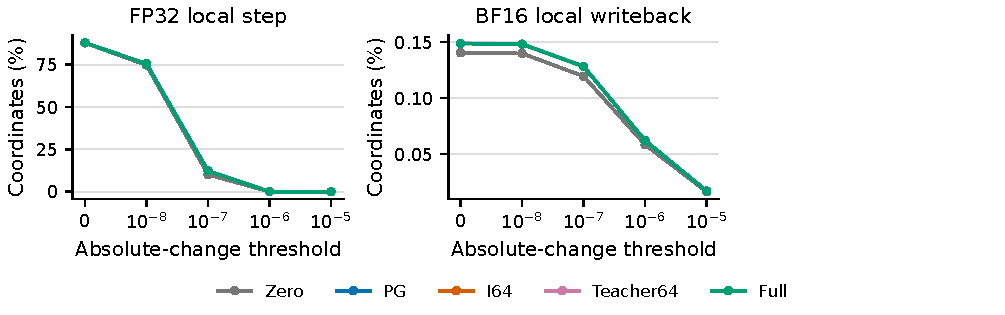
\includegraphics[width=\linewidth]{figures/aligned_evidence_20260910/thresholds.pdf}
\caption{Absolute-threshold sensitivity of the saved-state local steps. Lines show means over two banks and shading shows their range; the zero-gradient control has one value. The two panels use the same thresholds and separate FP32 master changes from BF16 writeback.}
\label{fig:thresholds}
\end{figure}

\subsection{Response banks, overlaps, and gradient magnitudes}
\label{app:gradient_overlap}

Banks use seeds 42 and 43, one response per domain per bank, a 2,048-token prompt cap, and a 256-token generation cap. All eight responses reach the cap. Four response positions are sampled without replacement per response. Each row's four prefixes receive equal weight. For routed gradients, each teacher scores its domain row; for common-bank gradients, it scores all four rows with equal domain weights. Crossed comparisons score every domain row with every teacher, keeping the number of prefixes per gradient at four. The 192 crossed-pair records and 48 routed/common pair records share underlying gradients, so points represent paired conditions within banks.

Top-$k$ coordinate sets rank absolute gradient values, using a stable coordinate index to break cutoff ties. The diagnostic records the cutoff and whether a tie crosses the selection boundary. These tie flags accompany the source metrics, including overlaps from nearly degenerate gradients. Table~\ref{tab:coverage_mass} supplies the routed PG norms; the first bank's instruction-following gradient has norm $1.53\times10^{-9}$. Cosine normalizes magnitude, so opposite directions for such a row carry very little absolute gradient mass. Jaccard overlap measures selected locations and cosine measures signed direction. For reference, independent uniform sets of fraction $\rho$ have expected-intersection to expected-union ratio $\rho/(2-\rho)$, or approximately 0.00503 at $\rho=1\%$. This reference uses uniform coordinates; layer and weight-magnitude structure remain in the measured gradients.

Applying Equation~\ref{subnet_overlap} to the largest-magnitude 1\% of raw-gradient coordinates gives the six-pair comparison in Figure~\ref{fig:teacher_overlap}. Across the two banks, routed gradients have mean Jaccard overlap 0.0951 for PG and 0.0999 for I64. Their ranges are 0.0744--0.1077 and 0.0737--0.1178. When every teacher instead scores all four domain responses, the respective means are 0.3808 and 0.4577. The latter comparison changes both input composition and prefix count; the crossed input control below fixes the count.

\begin{figure}[t]
\centering
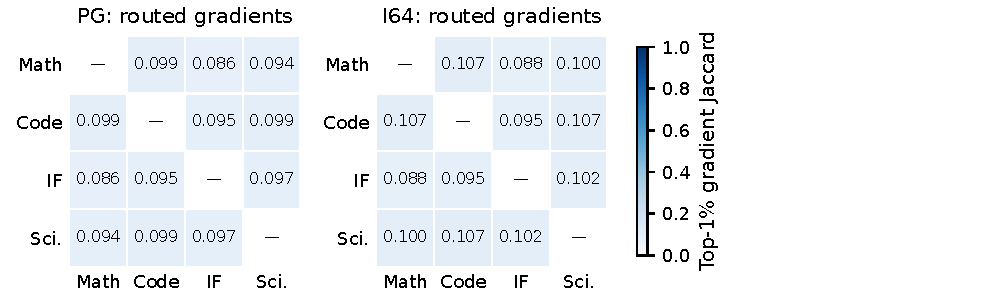
\includegraphics[width=\linewidth]{figures/aligned_evidence_20260910/teacher_overlap.pdf}
\caption{Teacher-pair raw-gradient comparison at M-PG update 100. Entries show mean Jaccard over two banks for the largest-magnitude 1\% of routed gradient coordinates. Both panels use the same scale.}
\label{fig:teacher_overlap}
\end{figure}

Holding the teacher fixed while changing the input domain yields mean gradient cosines of 0.0059 for PG and 0.0072 for I64. Holding the input domain fixed while changing teachers produces both aligned and opposed gradients. For routed gradients the mean cosines are $-0.0020$ and $0.0081$, respectively, despite partial coordinate overlap. Figure~\ref{fig:teacher} supplies this input and direction context for the teacher-overlap results in Section~\ref{sec:subnetworks}.

\begin{figure}[t]
\centering
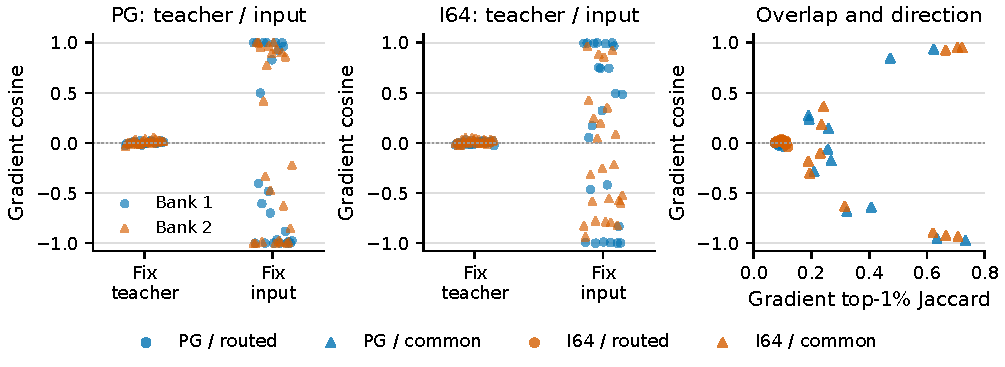
\includegraphics[width=\linewidth]{figures/aligned_evidence_20260910/teacher_input.pdf}
\caption{Supporting input controls for teacher overlap at M-PG update 100. Left and center: crossed comparisons keep four prefixes per gradient. Right: top-1\% gradient Jaccard versus signed cosine for routed and common-bank gradients. Dots share teachers and banks and are dependent comparisons.}
\label{fig:teacher}
\end{figure}

\section{Vocabulary Supervision and Coverage}
\label{app:losses}

\paragraph{Four-bank local experiment.}
The local supervision comparison in Figure~\ref{fig:density} uses four response banks with seeds 2042--2045 at M-PG update 100. Each bank contains one response per domain. Generation uses the training prompt format, a 2,048-token prompt cap, and a 4,096-token response cap. The 16 response lengths range from 81 to 4,096 tokens; two responses reach the cap. Six positions per response give 96 prefixes. PG actions are freshly sampled from the student at the cached prefixes. Every loss uses the same prefixes and domain-response weights. Gradients are globally clipped at norm 1 before applying the same saved Adam state.

The teacher-top-64 student probability mass averages 99.918\% across the 96 prefixes. The bank-domain averages range from 99.279\% to 100\%, and the lowest individual-prefix mass is 96.709\%. The source bundle records all 16 bank-domain coverage entries and every proposed update. Student BF16 values match the saved model exactly. The local loss and Adam implementations are the same as in the two-bank controls in Appendix~\ref{app:records}.


\paragraph{Implemented intersection loss.}
Let $S$ be the rollout student's top-64 set, $T$ the teacher's top-64 set, and $I=S\cap T$. The online I64 loss is
\begin{equation}
\ell_{\mathrm{I64}}=-\sum_{v\in I}\sg\!\left[
\frac{p_\theta(v)}{\sum_{u\in S}p_\theta(u)}
\bigl(\log q_d(v)-\log p_\theta(v)\bigr)\right]\log p_\theta(v).
\label{eq:i64}
\end{equation}
All probabilities use full-vocabulary normalization. Student weights are normalized over $S$ before masking to $I$; current student probabilities are recomputed at the saved candidate positions. An empty intersection contributes zero. PG uses detached log-ratio coefficients without advantage or policy-ratio clipping. I64 and PG are the online objectives used throughout the comparisons.

\paragraph{Teacher-top-64 local reference.}
The corrected teacher-top-64 diagnostic uses the fixed teacher set $T$ and full-vocabulary probabilities:
\begin{equation}
\ell_{\mathrm{T64}}=\sum_{v\in T}\left[p_\theta(v)\log\frac{p_\theta(v)}{q_d(v)}-p_\theta(v)+q_d(v)\right].
\label{eq:t64}
\end{equation}
Its gradient is $\sum_{v\in T}p_\theta(v)\log(p_\theta(v)/q_d(v))\nabla_\theta\log p_\theta(v)$. I64 instead uses the detached weights in Equation~\ref{eq:i64}, normalized over the original student set $S$. T64 and full vocabulary are local objective comparisons at the M-PG checkpoint; online capability curves compare PG and I64.

For a fixed prefix, differentiating Equation~\ref{eq:full} gives
\begin{align}
\nabla_\theta\ell_{\mathrm{full}}
&=\sum_{v\in\cV}p_\theta(v)\left(\log\frac{p_\theta(v)}{q_d(v)}+1\right)\nabla_\theta\log p_\theta(v)\\
&=\mathbb E_{a\sim p_\theta}\!\left[\log\frac{p_\theta(a)}{q_d(a)}\nabla_\theta\log p_\theta(a)\right],
\end{align}
using $\sum_v\nabla_\theta p_\theta(v)=0$. The identity conditions on prefixes and fixed weights. Original rollout losses additionally use the realized response and its eventual length-dependent weight. Table~\ref{tab:coverage_mass} reports the corresponding coverage for the two-bank controls used to interpret gradient overlap and optimizer history.

\begin{table}[t]
\caption{Coverage and routed gradient scale for the separate two-bank gradient and optimizer controls (256-token generation cap). Probability mass and full-vocabulary student entropy (nats) are averaged over each row's four prefixes. A displayed mass of 100\% may reflect rounding at the reported precision.}
\label{tab:coverage_mass}
\centering\small
\begin{tabular}{rlrrrr}
\toprule
Bank & Domain & Mass in $T$ (\%) & Mass in $I$ (\%) & Entropy & $\|g_{\mathrm{PG}}\|_2$ \\
\midrule
1 & Math & 100.0000 & 100.0000 & 0.3243 & 132.6 \\
1 & Code & 99.9968 & 99.9965 & 0.7701 & 163.8 \\
1 & IF & 100.0000 & 100.0000 & $1.85\times10^{-5}$ & $6.13\times10^{-9}$ \\
1 & Science & 99.9184 & 99.9162 & 0.7405 & 54.82 \\
2 & Math & 99.9991 & 99.9991 & 0.3221 & 2.605 \\
2 & Code & 100.0000 & 100.0000 & 0.2962 & 3.167 \\
2 & IF & 100.0000 & 100.0000 & 0.5004 & 55.52 \\
2 & Science & 99.9993 & 99.9992 & 0.2442 & 0.8505 \\
\bottomrule
\end{tabular}

\end{table}

\section{Teacher Distribution Distance}
\label{app:teacher_distance}

Teacher distance is computed on the full next-token vocabulary at matched prefixes:
\begin{equation}
\operatorname{JS}(q_d,q_e)=\tfrac12 D_{\mathrm{KL}}(q_d\|m)+\tfrac12 D_{\mathrm{KL}}(q_e\|m),
\qquad m=\tfrac12(q_d+q_e).
\label{eq:teacher_js}
\end{equation}
We average over the same equally weighted domains and prefixes for every pair. Figure~\ref{fig:teacher_js} pairs all twelve bank-pair JS measurements with their corresponding gradient overlaps. Teacher JS ranges from 0.00151 to 0.02714 nats. Routed gradient-selection differences lie in a narrow band, while common-input differences vary more widely. The ordering of teacher pairs changes with the input bank and supervision choice. These pairwise observations share teachers, prefixes, and a student checkpoint.

\begin{figure}[t]
\centering
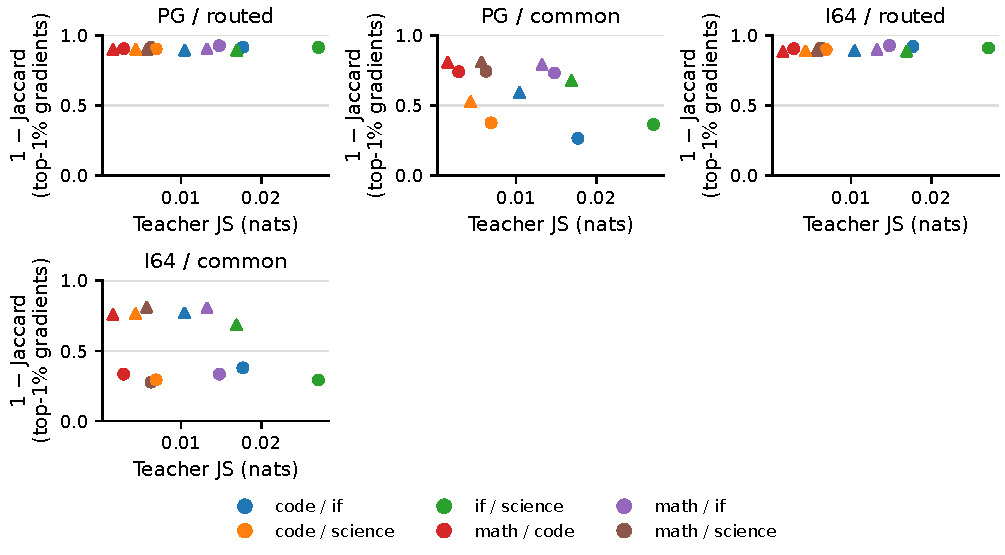
\includegraphics[width=\linewidth]{figures/aligned_evidence_20260910/teacher_js.pdf}
\caption{Teacher prediction differences and raw-gradient selection differences at M-PG update 100. Colors identify the six teacher pairs; circles and triangles identify the two banks. Each panel pairs the same teacher JS values with PG or I64 gradient overlap on routed or common inputs.}
\label{fig:teacher_js}
\end{figure}

\section{Token Shares Under the Three Averaging Rules}
\label{app:behavior}

Figure~\ref{fig:all_token_shares} supports the loss-weighting comparison in Section~\ref{sec:normalization}. Each branch allocates 25\% of prompts to every domain. Under GT, the plotted token shares also give the domain loss weights. DT and DR fix those weights to 25\% even when generated token shares differ. Records at the same rollout clock are merged across metric writes before plotting; the plot shows the common first 50 rollout batches without smoothing, matching the capability comparison in Section~\ref{sec:normalization}. Longer histories remain in the source bundle.

\begin{figure}[t]
\centering
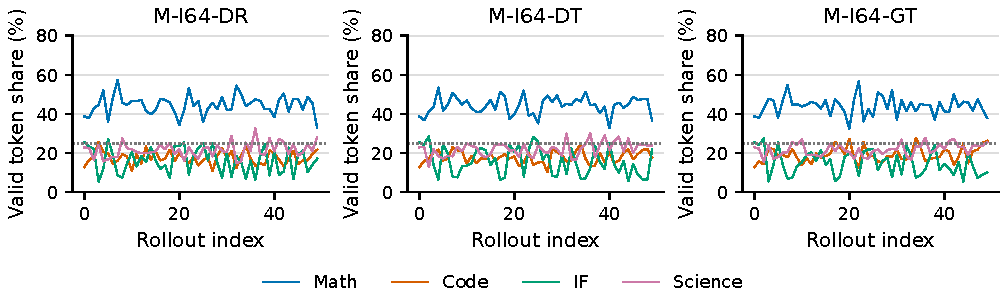
\includegraphics[width=\linewidth]{figures/aligned_evidence_20260910/all_token_shares.pdf}
\caption{Valid-token shares over the first 50 rollout batches for mathematics, code, instruction following, and science under the three I64 reductions. The dotted reference is the common 25\% prompt share. Rollout index $r$ precedes optimizer update $r+1$. GT uses these shares as domain loss weights; DT and DR use fixed domain weights.}
\label{fig:all_token_shares}
\end{figure}
